Struktureller Aufbau des Projektes.

\tikzstyle{myNode20} = [draw=black, fill=black!20,
    rectangle, inner sep=5pt, inner ysep=5pt]
\tikzstyle{myNode15} = [draw=black, fill=black!15,
    rectangle, inner sep=5pt, inner ysep=5pt]
\tikzstyle{myNode10} = [draw=black, fill=black!10,
    rectangle, inner sep=5pt, inner ysep=5pt, text width=5cm]
\tikzstyle{myNode5} = [draw=black, fill=black!5,
    rectangle, inner sep=5pt, inner ysep=5pt, text width=3cm]
\tikzstyle{myNode0} = [draw=white, fill=white,
    rectangle, inner sep=5pt, inner ysep=5pt]

\begin{center}
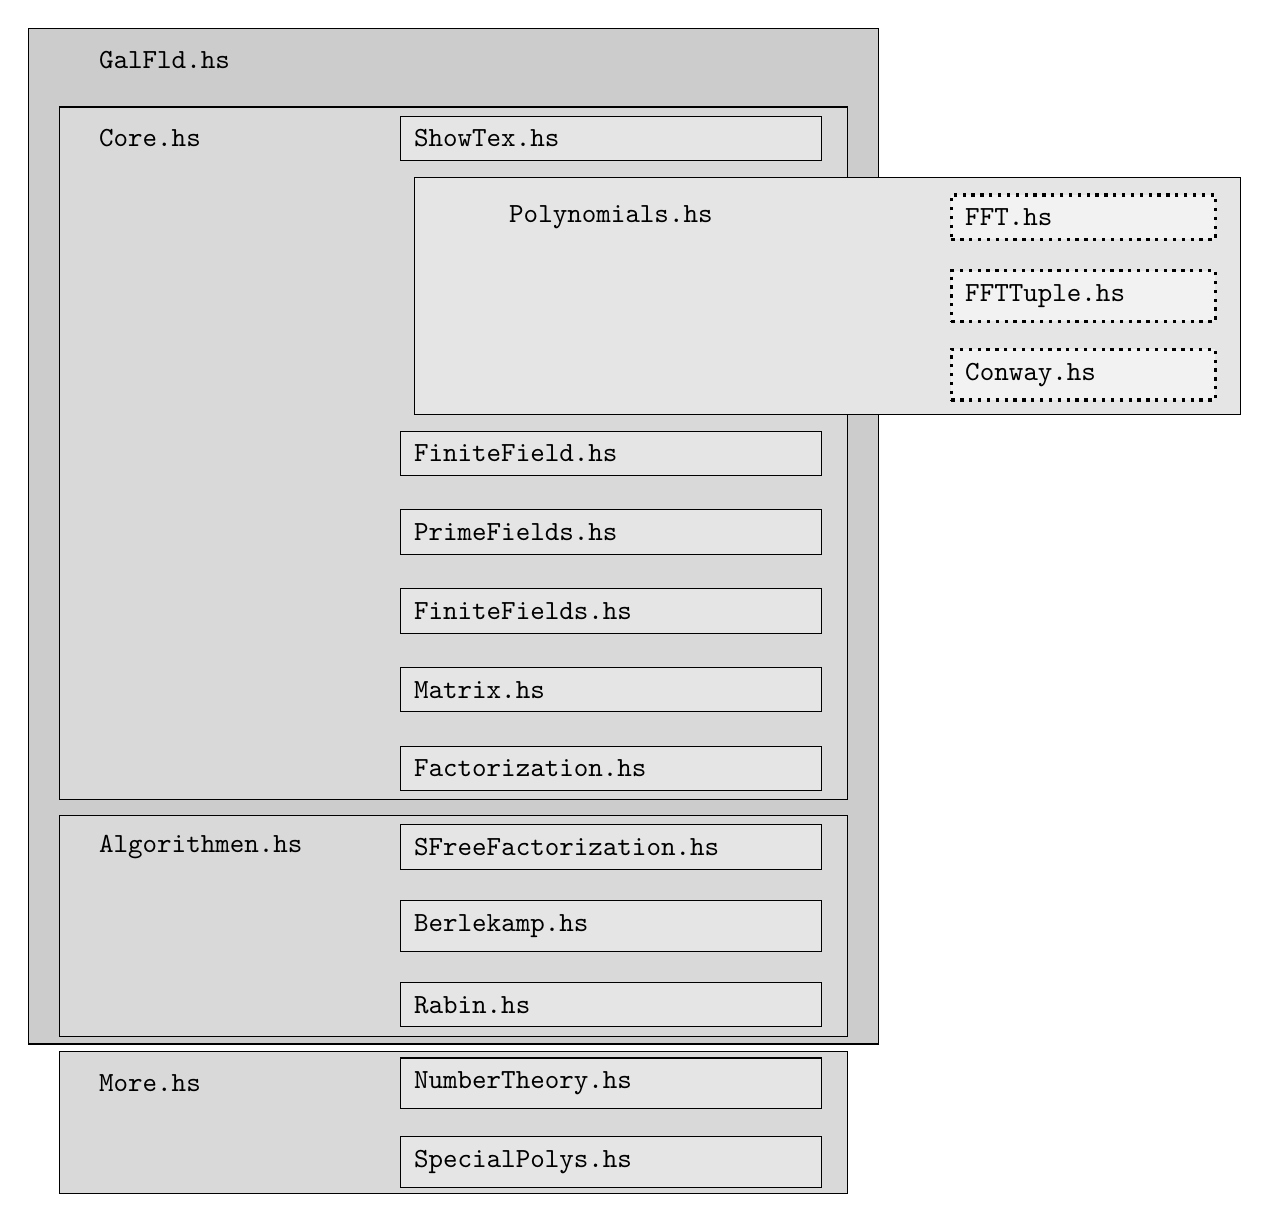
\begin{tikzpicture}

\draw[myNode20] (-2.4,1.4) rectangle (8.4,-11.5);
\draw[myNode15] (-2,0.4) rectangle (8,-8.4);
\draw[myNode15] (-2,-8.6) rectangle (8,-11.4);
\draw[myNode15] (-2,-11.6) rectangle (8,-13.4);
\draw[myNode10] (2.5,-0.5) rectangle (13,-3.5);

\node[text width=3cm] (GalFld) at (0,1) [] {\texttt{GalFld.hs}};
\node[text width=3cm] (Core) at (0,0) [] {\texttt{Core.hs}};
  \node[myNode10] (ShowTex) at (5,0) [] {\texttt{ShowTex.hs}};
  \node (Polynomials) at (5,-1) [] {\texttt{Polynomials.hs}};
    \node[myNode5,dotted,very thick] (FFT) at (11,-1) [] {\texttt{FFT.hs}};
    \node[myNode5,dotted,very thick] (FFTTuple) at (11,-2) {\texttt{FFTTuple.hs}};
    \node[myNode5,dotted,very thick] (Conway) at (11,-3) {\texttt{Conway.hs}};
  \node[myNode10] (FiniteField) at (5,-4) [] {\texttt{FiniteField.hs}};
  \node[myNode10] (PrimeFields) at (5,-5) [] {\texttt{PrimeFields.hs}};
  \node[myNode10] (FiniteFields) at (5,-6) [] {\texttt{FiniteFields.hs}};
  \node[myNode10] (Matrix) at (5,-7) [] {\texttt{Matrix.hs}};
  \node[myNode10] (Factorization) at (5,-8) [] {\texttt{Factorization.hs}};
\node[text width=3cm] (Algorithmen) at (0,-9) [] {\texttt{Algorithmen.hs}};
  \node[myNode10] (SFreeFactorization) at (5,-9) []
    {\texttt{SFreeFactorization.hs}};
  \node[myNode10] (Berlekamp) at (5,-10) [] {\texttt{Berlekamp.hs}};
  \node[myNode10] (Rabin) at (5,-11) [] {\texttt{Rabin.hs}};
\node[text width=3cm] (More) at (0,-12) [] {\texttt{More.hs}};
  \node[myNode10] (NumberTheory) at (5,-12) [] {\texttt{NumberTheory.hs}};
  \node[myNode10] (SpecialPolys) at (5,-13) [] {\texttt{SpecialPolys.hs}};
\end{tikzpicture}
\end{center}
